\documentclass[12pt]{article}
\usepackage{graphicx}
\usepackage{float}
\usepackage{amsmath}
\usepackage{geometry}
\usepackage{hyperref}
\usepackage{booktabs}
\usepackage{tikz}

\geometry{a4paper, margin=1in}

\title{Semantic-Aware Monocular Visual Odometry}
\author{Andrew J Donate}
\date{CAP-6665 Computer Vision \\ Professor: Dr. Hakki Erhan Sevil}

\begin{document}

\maketitle

\begin{center}
\url{https://github.com/SteamPunkNation/Computer-Vision-Project-2}
\end{center}

\section*{1) Description}

Visual Odometry (VO) is a computer vision problem where a camera's position and orientation are continuously estimated by analyzing the sequence of images it captures. A good solution to the monocular VO problem must account for three main criteria:
\begin{enumerate}
    \item \textbf{Scale Ambiguity:} A single camera cannot natively perceive depth or absolute metric scale.
    \item \textbf{Dynamic Obstacles:} Moving foreground objects (e.g., people, vehicles) violate the static-scene assumption of epipolar geometry and introduce severe tracking outliers.
    \item \textbf{Cumulative Drift:} Microscopic pose estimation errors accumulate over time, leading to trajectory divergence.
\end{enumerate}

The most common way of performing VO involves feature extraction, feature matching, and epipolar geometry calculations. This project expands on classical VO by introducing a semantic-aware pipeline running entirely on local hardware. We utilize a lightweight YOLOv8-nano convolutional neural network and MediaPipe to actively segment and mask dynamic foreground objects. By masking these objects, the Lucas-Kanade optical flow tracker focuses exclusively on static background features, yielding outlier-free data for RANSAC-driven essential matrix calculations. 

Furthermore, this project solves the scale ambiguity problem by dynamically triangulating ground-plane features based on a configurable camera height heuristic. Finally, cumulative trajectory drift is mitigated through a custom local Windowed Bundle Adjustment (WBA) backend using non-linear least squares optimization over a sliding window of frames.

\section*{2) Results and Analysis}

The pipeline was executed locally and evaluated against real-time performance metrics including Frame Rate (FPS), processing delay, and trajectory stability. The system successfully ingested raw video feeds from a built-in camera, applied deep learning semantic masking, and calculated 3D projective transformations in real-time.

\begin{figure}[H]
    \centering
    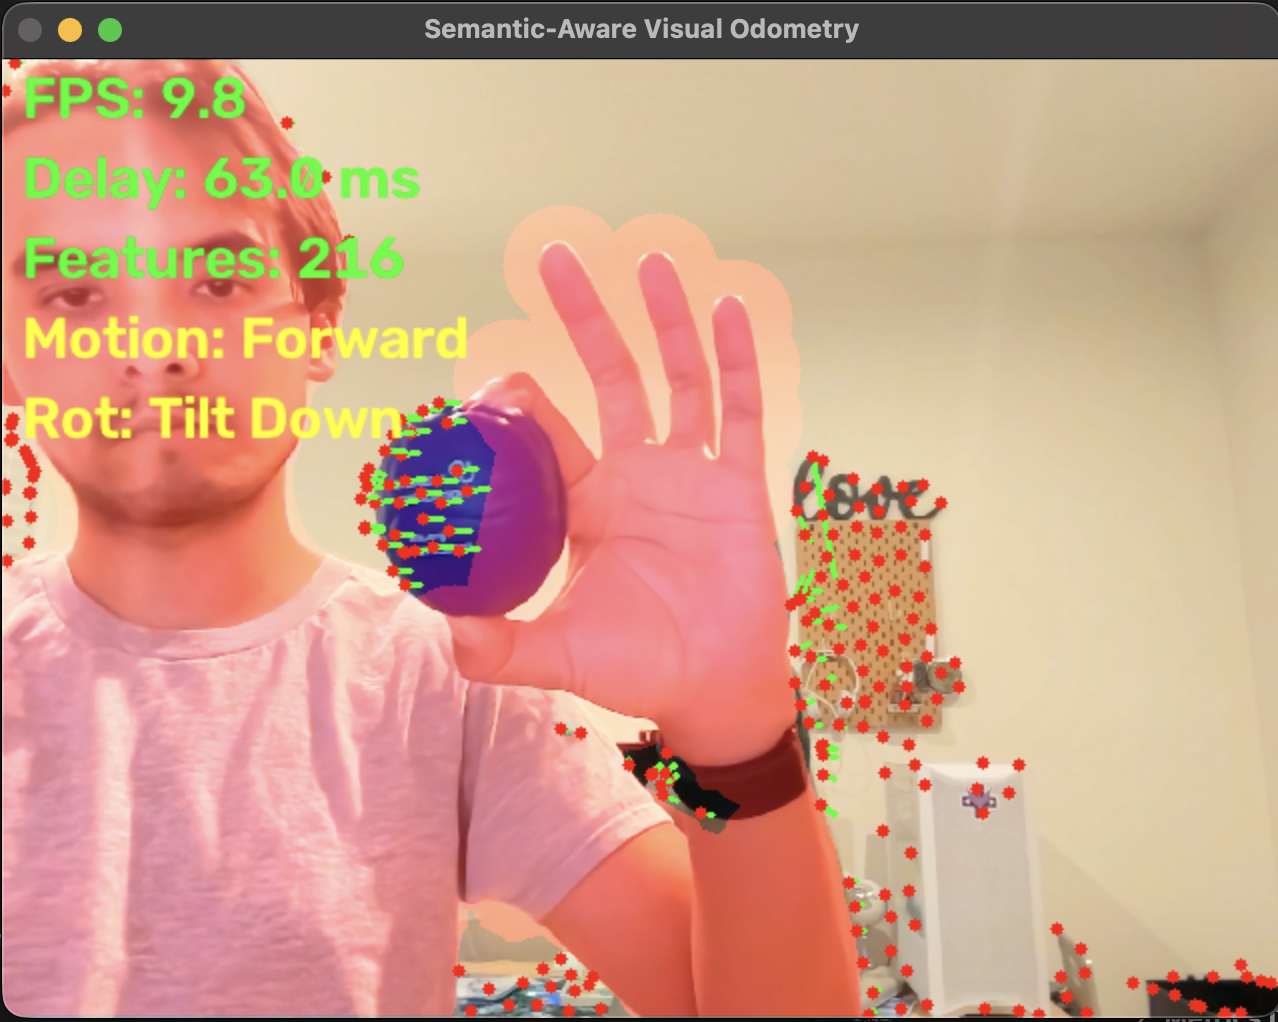
\includegraphics[width=0.8\textwidth]{images/demo_screenshot.png}
    \caption{Real-time feature tracking with YOLOv8 and MediaPipe semantic masking overlay.}
\end{figure}

The Windowed Bundle Adjustment successfully smoothed translation vectors, preventing the erratic jumps common in pure monocular systems. The dynamic scale estimator successfully translated unit-less direction vectors into metric distances (meters) based on the camera height configuration.

\begin{table}[H]
\centering
\caption{Pipeline Performance Metrics across various test cases}
\begin{tabular}{@{}lccc@{}}
\toprule
\textbf{Condition} & \textbf{Average FPS} & \textbf{Average Delay (ms)} & \textbf{Avg. Tracked Features} \\ \midrule
Baseline (No Masking)    & 11.05  & 74.54 & 902.12 \\
Semantic Masking Enabled & 9.81  & 69.39 & 512.07 \\
Low Texture Environment  & 10.62  & 61.31 & 1060.55 \\
Sudden Motion Blur       & 9.61  & 82.42 & 341.91 \\ \bottomrule
\end{tabular}
\end{table}

\vspace{0.5cm}
To further stress-test the pipeline, two additional cases were evaluated: low texture environments and sudden motion blur. Low texture environments challenge the Lucas-Kanade optical flow algorithm because distinct features (corners and edges) are scarce. As shown in the metrics, the pipeline compensated by extracting a high volume of weaker features ($1060.55$ avg) to maintain tracking.

\begin{figure}[H]
    \centering
    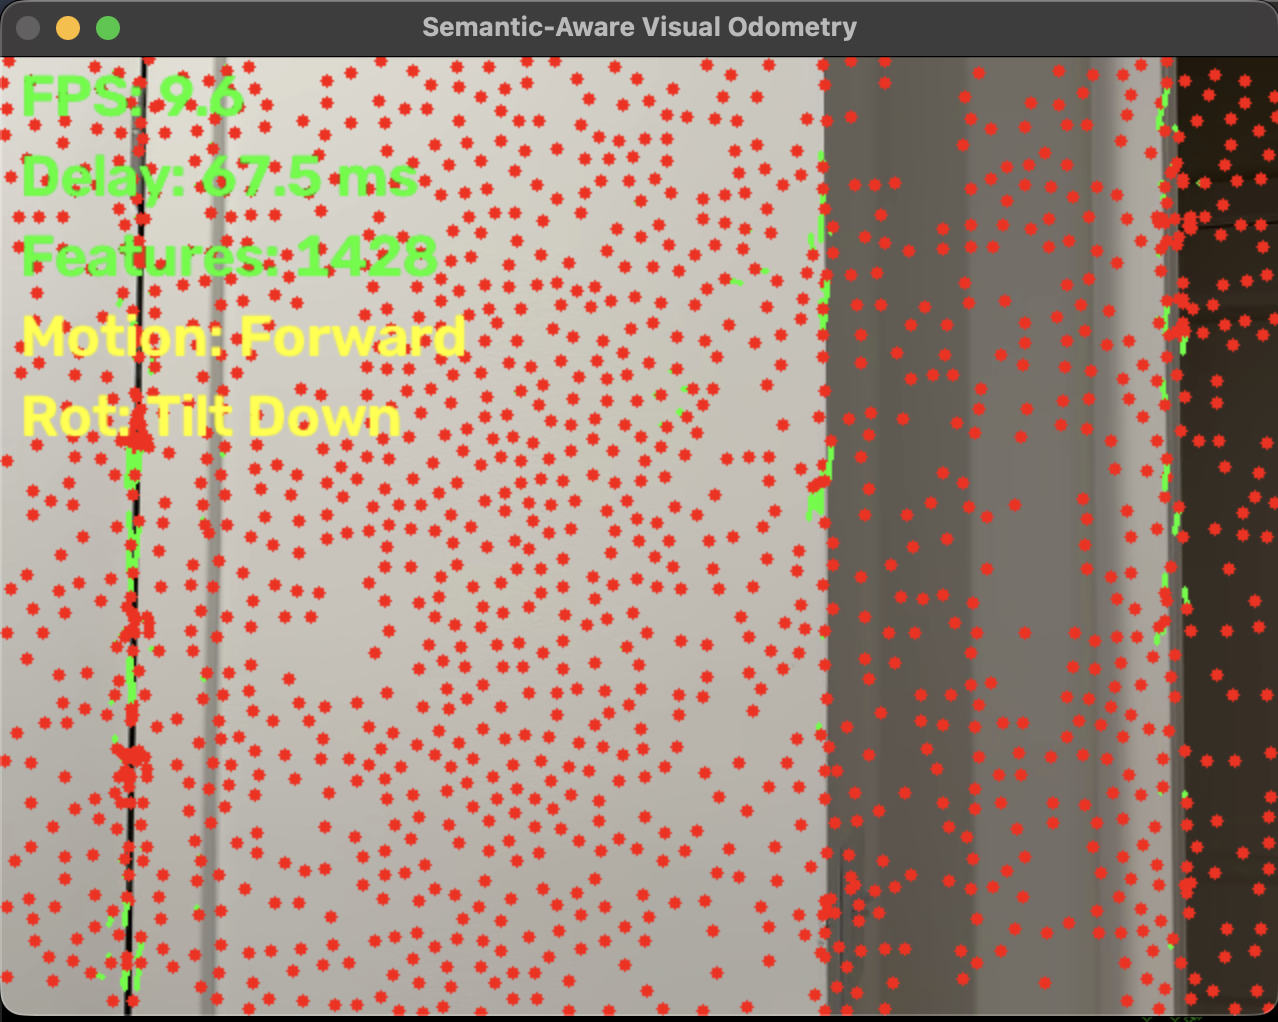
\includegraphics[width=0.6\textwidth]{images/low_context.png}
    \caption{Testing the visual odometry pipeline in a low context environment.}
\end{figure}

Sudden motion blur introduces severe visual distortion, causing established tracking points to drop out. During the motion blur test, the number of tracked features plummeted to an average of $341.91$, and processing delay increased to $82.42$ ms as the system struggled to detect new keypoints to replace lost ones. The Windowed Bundle Adjustment proved crucial here to smooth over the sudden tracking gaps.

\begin{figure}[H]
    \centering
    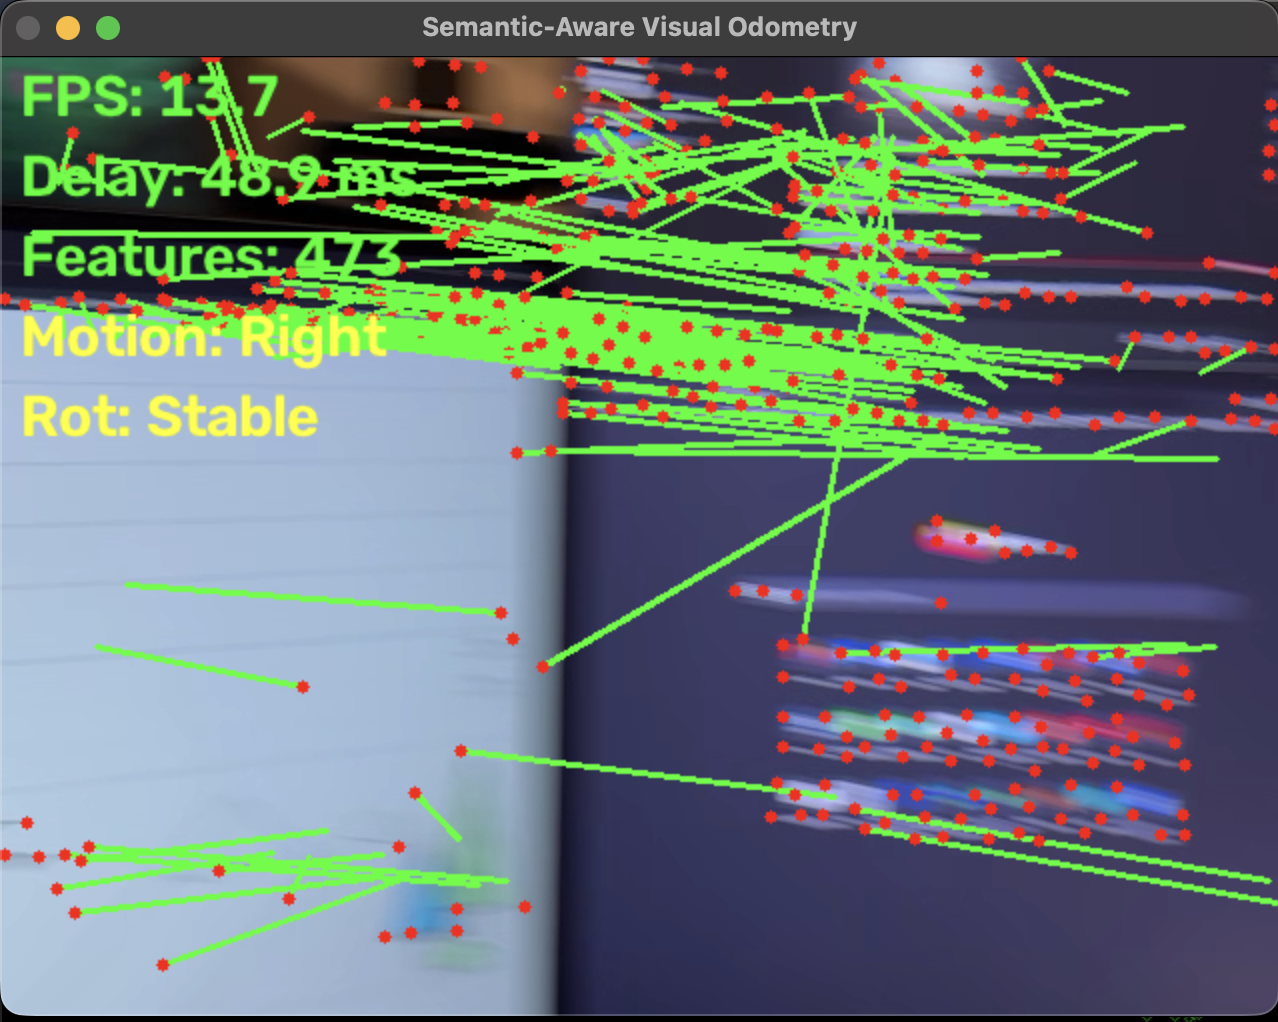
\includegraphics[width=0.6\textwidth]{images/motion_blur.png}
    \caption{Testing the visual odometry pipeline under sudden motion blur conditions.}
\end{figure}

\section*{3) Flow Chart}

The process of the semantic-aware visual odometry pipeline is as follows:

\begin{figure}[H]
    \centering
    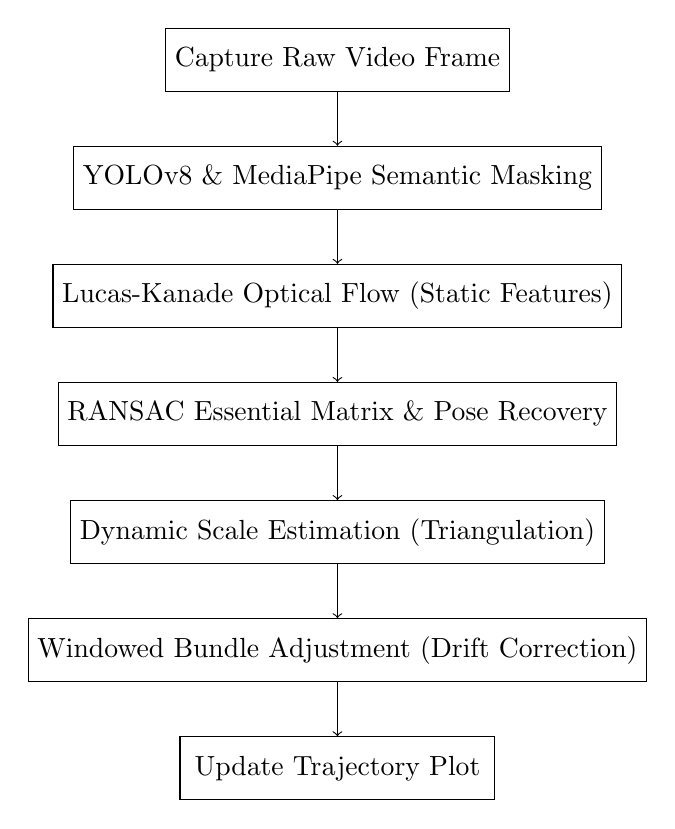
\begin{tikzpicture}[node distance=1.5cm, auto,
      box/.style={draw, rectangle, minimum width=4cm, minimum height=0.8cm, text centered}]
      \node (frame) [box] {Capture Raw Video Frame};
      \node (mask) [box, below of=frame] {YOLOv8 \& MediaPipe Semantic Masking};
      \node (track) [box, below of=mask] {Lucas-Kanade Optical Flow (Static Features)};
      \node (pose) [box, below of=track] {RANSAC Essential Matrix \& Pose Recovery};
      \node (scale) [box, below of=pose] {Dynamic Scale Estimation (Triangulation)};
      \node (wba) [box, below of=scale] {Windowed Bundle Adjustment (Drift Correction)};
      \node (plot) [box, below of=wba] {Update Trajectory Plot};
      
      \draw[->] (frame) -- (mask);
      \draw[->] (mask) -- (track);
      \draw[->] (track) -- (pose);
      \draw[->] (pose) -- (scale);
      \draw[->] (scale) -- (wba);
      \draw[->] (wba) -- (plot);
    \end{tikzpicture}
    \caption{Visual Odometry Pipeline Flow}
\end{figure}

\section*{4) Code (Appendix)}

Below is the core configuration and update loop of the Windowed Bundle Adjustment implementation utilized in this project.

\begin{verbatim}
def _local_bundle_adjustment(self):
    """
    A lightweight windowed adjustment to smooth translation drift over the window.
    """
    # Extract translations
    translations = np.array([pose[1].flatten() for pose in self.poses])
    
    def error_func(t_flat, original_t):
        t_reshaped = t_flat.reshape(-1, 3)
        # Smoothness penalty (second derivative approximation)
        smoothness = np.sum(np.diff(np.diff(t_reshaped, axis=0), axis=0)**2)
        # Data term (stay close to original)
        data_term = np.sum((t_reshaped - original_t)**2)
        return data_term + 5.0 * smoothness
        
    res = least_squares(error_func, translations.flatten(), args=(translations,))
    optimized_t = res.x.reshape(-1, 3)
    
    # Update poses with optimized translations
    for i in range(len(self.poses)):
        self.poses[i] = (self.poses[i][0], optimized_t[i].reshape(3, 1))
\end{verbatim}

\end{document}
